\documentclass[11pt, twoside]{book}     % Definimos el tipo de documento

%% Paquetes y configuraciones
    % Paquetes de Formato y Tipografía
        \usepackage[T1]{fontenc}            % Codificación de fuente que mejora la salida en PDF
        \usepackage[utf8]{inputenc}         % Permite el uso de caracteres especiales (tildes, ñ, etc.)
        \usepackage[letterpaper,lmargin=3cm,rmargin=2cm,top=2cm,bottom=2cm]{geometry}
        \usepackage{times}                  % Usa la fuente Times New Roman
        \hyphenation{co-mer-cial rea-li-zan si-guien-te si-mu-la-ción ke-lly con-si-de-ra-da}                   % Silabeo de palabras
        \usepackage{titlesec}
        \usepackage{fancyhdr}               % Encabezados y pies de página
        \usepackage{tikz}                   % Paquete para gráficos vectoriales


    % Paquetes de Idioma
        \usepackage[spanish]{babel}         % Configura el idioma a español (traduce títulos, orden de palabras, etc.)
        \spanishdecimal{.}                  % Establece el punto como separador decimal en español

    % Paquetes Matemáticos
        \usepackage{amsmath}      % Soporte para ecuaciones matemáticas avanzadas
        \usepackage{amssymb}      % Símbolos matemáticos adicionales
        \usepackage{mathrsfs}     % Fuente matemática caligráfica

    % Paquetes para Figuras y Tablas
        \usepackage{graphicx}      % Permite incluir imágenes en el documento
        \usepackage{float}         % Controla la posición de imágenes y tablas
        \usepackage{subfigure}     % Permite incluir subfiguras dentro de una figura
        \usepackage{tabularx}      % Mejora el control de tablas con ancho ajustable
        \usepackage[table]{xcolor} % Permite usar colores en tablas

    % Paquetes de Hipervínculos y Referencias
        \usepackage{natbib}                           % Manejo de referencias bibliográficas
        \usepackage[colorlinks=true, allcolors=blue]{hyperref} % Habilita enlaces internos y externos en color azul
        \bibpunct{(}{)}{;}{a}{,}{,}                  % Configuración del formato de citas

    % Paquetes para formato de Código Fuente
        \usepackage{listingsutf8}     % Paquete para mostrar código fuente con sintaxis destacada
        \definecolor{codegreen}{rgb}{0,0.6,0}  % Color para comentarios en código
        \definecolor{codegray}{rgb}{0.5,0.5,0.5} % Color para números de línea
        \definecolor{codepurple}{rgb}{0.58,0,0.82} % Color para cadenas de texto
        \definecolor{backcolour}{rgb}{0.95,0.95,0.92} % Color de fondo para bloques de código

        \lstdefinestyle{mystyle} 
        {
            frame=single,                       % Marco alrededor del código
            backgroundcolor=\color{white},      % Fondo blanco
            commentstyle=\color{codegreen},     % Comentarios en verde
            keywordstyle=\color{magenta},       % Palabras clave en magenta
            numberstyle=\tiny\color{codegray},  % Números de línea en gris
            stringstyle=\color{codepurple},     % Cadenas en púrpura
            basicstyle=\ttfamily\footnotesize,  % Fuente monoespaciada pequeña
            breaklines=true,                    % Permitir saltos de línea en código
            captionpos=b,                       % Coloca los títulos del código abajo
            numbers=left,                       % Números de línea a la izquierda
            tabsize=2                           % Espaciado de tabulación de 2
        }
        \lstset{style=mystyle}                  % Aplica el estilo definido
        \lstset{inputencoding=utf8/latin1}      % Permite caracteres especiales en código

    % Paquetes para Diagramas y Gráficos
        \usepackage{tikz}                           % Paquete para gráficos vectoriales
        \usetikzlibrary{shapes.geometric, arrows}   % Librerías de TikZ para diagramas de flujo

    % Definición de estilos de nodos y flechas en diagramas de flujo
        \tikzstyle{process} = [rectangle, minimum width=3cm, minimum height=1cm, text centered, draw=black]
        \tikzstyle{arrow} = [thick,->,>=stealth]

    % Estilo de los títulos de los capítulos    
        \titleformat{\chapter}[frame]{\normalfont}{\filcenter \small \ CAPÍTULO \  \thechapter \ }{10pt}{\Large\bfseries\filcenter}

    % Estilo de los títulos de las secciones    
        \titleformat{\section}[display] {}{\filcenter\bfseries Sección \thesection.}{0pt}{\titlerule[1pt] \itshape\fillast}[{\titlerule[1pt]}]

    % Configuración del encabezado
        \pagestyle{fancy}                   % Establece el estilo de la página
        \fancyhf{}                          % Limpia el encabezado y pie de página
        \fancyhead[LE,RO]{\thepage}         % Números de página en las esquinas
        \fancyhead[RE]{\leftmark}           % Capítulo en la esquina superior derecha
        \fancyhead[LO]{\rightmark}          % Sección en la esquina superior izquierda
        \renewcommand{\headrulewidth}{0.5pt} % Línea horizontal en la parte superior de la página
        \renewcommand{\footrulewidth}{0pt}   % Línea horizontal en la parte inferior de la página

% Macros para palabras importantes
    \newcommand{\fullname}      {Control de un Péndulo Invertido sobre Dos Ruedas Seguidor de Línea mediante Aprendizaje basado en Series de Fourier}
    \newcommand{\docdate}       {15 de marzo del 2025}
    
    \newcommand{\balancin}      {PISDRSL}
    \newcommand{\sistcontrol}   {FSLC}
    
%---------------------------------------------------------------------%

\begin{document}

    %----------------- PORTADA -----------------%
    \begin{titlepage}
        \thispagestyle{empty}
        \begin{minipage}[c][0.17\textheight][c]{0.25\textwidth}
            \begin{center}
                
\includegraphics[height=4cm]{Recursos/Imagenes/Portada/Escudo_UAQ.png}
            \end{center}
        \end{minipage}
        \begin{minipage}[c][0.195\textheight][t]{0.75\textwidth}
            \begin{center}
                \vspace{0.3cm}
                \textsc{\large UNIVERSIDAD AUTÓNOMA DE QUERÉTARO}\\[0.5cm]
                \vspace{0.3cm}
                \hrule height2.5pt
                \vspace{.2cm}
                \hrule height1pt
                \vspace{.8cm}
                \textsc{ FACULTAD DE INGENIERIA }\\[0.5cm] %
            \end{center}
        \end{minipage}

        \begin{minipage}[c][0.81\textheight][t]{0.25\textwidth}
            \vspace*{5mm}
            \begin{center}
                \hskip2.0mm
                \vrule width1pt height13cm 
                \vspace{5mm}
                \hskip2pt
                \vrule width2.5pt height13cm
                \hskip2mm
                \vrule width1pt height13cm \\
                \vspace{5mm}
                
\includegraphics[height=4.0cm]{Recursos/Imagenes/Portada/Escudo_Ingenieria_UAQ.png}
            \end{center}
        \end{minipage}
        \begin{minipage}[c][0.81\textheight][t]{0.75\textwidth}
            \begin{center}
                \vspace{1cm}

                {\large\scshape \fullname}\\[.2in]

                \vspace{1.5cm}            

                \textsc{\LARGE T\hspace{1.5cm}E\hspace{1.5cm}S\hspace{1.5cm}I\hspace{1.5cm}S}\\[1cm]
                \textsc{\large para obtener el grado de:}\\[0.5cm]
                \textsc{\large Ingeniero en Automatización}\\[1.5cm]
                \textsc{\large presenta:}\\[0.5cm]
                \textsc{\large {Diego Joel Zuñiga Fragoso}}\\[1.5cm]          

                {\large\scshape Directores de tesis:\\[0.3cm] {Director 1 \\[0.2cm]
        
                Director 2}}\\[1.5cm]

                \large{QUERÉTARO, QRO.} {A MARZO DEL} {2025}
            \end{center}
        \end{minipage}
    \end{titlepage}
    \newpage
    
    \tableofcontents        % Índice en números romanos
    \thispagestyle{empty}   % Elimina la numeración en la página del índice
    \newpage

    \listoffigures          % Lista de figuras
    \thispagestyle{empty}   % Elimina la numeración en la página del índice
    \newpage
    
    \listoftables           % Lista de tablas
    \thispagestyle{empty}   % Elimina la numeración en la página del índice
    \newpage

    \pagenumbering{arabic}  % Cambio a números arábigos en el contenido principal
    \setcounter{page}{1}   % Asegura que comience desde "1

    %----------------- RESUMEN -----------------%
    \chapter{Resumen}

    %----------------- INTRODUCCION -----------------%
    \chapter{Introducción}
        \section{Planteamiento del problema}

        \section{Objetivos generales}

        \section{Objetivos específicos}


    %----------------- MARCO TEORICO -----------------%
    \chapter{Fundamentación Teórica}  

        \section{Modelo no lineal del péndulo con dos ruedas}

            El diagrama esquemático con sus marcos referenciales y principales convenciones del péndulo con dos ruedas se muestra en la Figura \ref{Figura1}:

            \begin{figure}[H]
                \centering
                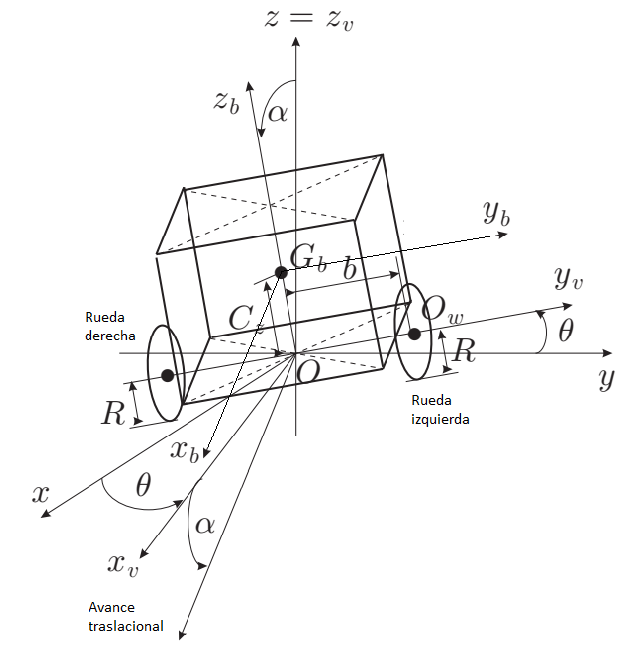
\includegraphics[width=0.6\textwidth]{Recursos/Imagenes/Fundamentacion_teorica/Diagrama_modelo_dinamico.png}
                \caption{Péndulo con dos ruedas.} 
                \label{Figura1}
            \end{figure}
    
            El modelo dinámico no lineal del péndulo con dos ruedas obtenido con las ecuaciones de Euler-Lagrange está dado por \citep{VMHGuzmancontrol2013}:
    
            \begin{equation}
                M(q)\ddot{q}+C(q,\dot{q})\dot{q}+g(q)= \ B(q)\tau
                \label{eq:formula1}
            \end{equation}
    
            \begin{equation}
                q=[x_0 \ \ y_0 \ \ \theta \ \ \alpha \ \ \phi_r \ \ \phi_l]^{T}
            \end{equation}
    
            \begin{equation}	
                M(q) =
                \begin{bmatrix}
                    M_p(1 + \tan^2(\beta)) & 0 & \Delta_1 & \Delta_2 & 0 & 0 \\
                    0 & M_p & \Delta_3 & \Delta_4 & 0 & 0 \\
                    \Delta_1 & \Delta_3 & \Delta_5 & 0 & 0 & 0 \\
                    \Delta_2 & \Delta_4 & 0 & M_p C_z^2 + I_{yy} & 0 & 0 \\
                    0 & 0 & 0 & 0 & M_w R^2 + I_{wa} & 0 \\
                    0 & 0 & 0 & 0 & 0 & M_w R^2 + I_{wa}
                \end{bmatrix}
            \end{equation}

            \begin{equation}
                \Delta_1 = -M_p C_z\sin(\alpha)\sin(\theta)
            \end{equation}

            \begin{equation}
                \Delta_2 = M_p C_z(\cos(\alpha)\cos(\theta)-\sin(\alpha)\tan(\beta))
            \end{equation}

            \begin{equation}
                \Delta_3 = M_p C_z\sin(\alpha)\cos(\theta)
            \end{equation}

            \begin{equation}
                \Delta_4 = M_p C_z\cos(\alpha)\sin(\theta)
            \end{equation}

            \begin{equation}
                \Delta_5 = (M_pC_z^{2}+I_{xx})\sin^{2}(\alpha)+I_{zz}\cos^{2}(\alpha)+2I_{\omega d}
            \end{equation}

            \begin{equation}
            C(q, \dot{q}) =
            \begin{bmatrix}
                0 & 0 & \Gamma_1 & \Gamma_2 & 0 & 0 \\
                0 & 0 & \Gamma_3 & \Gamma_4 & 0 & 0 \\
                0 & 0 & \Gamma_5 & \Gamma_6 & 0 & 0 \\
                0 & 0 & -\Gamma_6 & 0 & 0 & 0 \\
                0 & 0 & 0 & 0 & 0 & 0 \\
                0 & 0 & 0 & 0 & 0 & 0
            \end{bmatrix}
            \end{equation}

            \begin{equation}
                \Gamma_1= -M_pC_z(\dot{\theta}\sin(\alpha)\cos(\theta)+\dot{\alpha}\sin(\theta)\cos(\alpha))
            \end{equation}

            \begin{equation}
                \Gamma_2= -M_pC_z(\dot{\theta}\sin(\theta)\cos(\alpha)+\dot{\alpha}\sin(\alpha)\cos(\theta)+\dot{\alpha}\cos(\alpha)\tan(\beta))
            \end{equation}

            \begin{equation}
                \Gamma_3= -M_pC_z(\dot{\theta}\sin(\alpha)\sin(\theta)-\dot{\alpha}\cos(\alpha)\cos(\theta))
            \end{equation}

            \begin{equation}
                \Gamma_4= M_pC_z(\dot{\theta}\cos(\alpha)\cos(\theta)-\dot{\alpha}\sin(\alpha)\sin(\theta))
            \end{equation}

            \begin{equation}
                \Gamma_5= (M_pC_z^{2}+I_{xx}-I_{zz})\dot{\alpha}\sin(\alpha)\cos(\alpha)
            \end{equation}

            \begin{equation}
                \Gamma_6= (M_pC_z^{2}+I_{xx}-I_{zz})\dot{\theta}\sin(\alpha)\cos(\alpha)
            \end{equation}


            \begin{equation}
                g(q) =
                \begin{bmatrix}
                    (M_p+2M_\omega)g\tan(\beta) \\
                    0 \\
                    0 \\
                    -M_pC_zg\sin(\alpha) \\
                    0  \\
                    0 
                \end{bmatrix}
            \end{equation}

            \begin{equation}
                B(q) =
                \begin{bmatrix}
                    0 & 0 \\
                    0 & 0 \\
                    0 & 0 \\
                    -1 & -1 \\
                    1 & 0  \\
                    0 & 1
                \end{bmatrix}
            \end{equation}

            \begin{equation}
                \tau =
                \begin{bmatrix}
                    \tau_r\\
                    \tau_l
                \end{bmatrix}
            \end{equation}

            \noindent donde las coordenadas del punto $O$ son $ (x_o, y_o) $, $ \beta $ es el ángulo de una pendiente que sube el robot al avanzar, $ R $ es el radio de la rueda, $ g = 9.81 \ [\frac{m}{s^2}] $ es la aceleración de la gravedad, $ M_p $ es la masa del péndulo, $ C_z $ es la distancia del centro de masa del péndulo al punto $O$, $ b $ es la distancia del punto $O$ al punto $ O_w $, $ I_{xx} $ es el momento de inercia calculado alrededor del eje $ x_b $, $ I_{yy} $ es el momento de inercia calculado alrededor del eje $ y_b $, $ I_{zz} $ es el momento de inercia calculado alrededor del eje $ z_b $, $ I_{wd} $ es el momento de inercia de la rueda alrededor de su diámetro, $ I_{wa} $ es el momento de inercia de la rueda alrededor de su eje, $ M_w $ es la masa completa de la rueda (llanta, rin, cople y rotor),$ \ \phi_r $ es el ángulo de rotación de la rueda derecha, $ \phi_l $ es el ángulo de rotación de la rueda izquierda, $ \alpha $ es el ángulo de inclinación del péndulo, $ \theta $ es el ángulo de orientación del robot y $ v $ es la velocidad traslacional del robot dada como:

            \begin{equation}
                v= \frac{R}{2}(\dot{\phi_r}+\dot{\phi_l})
            \end{equation}

            La velocidad de orientación del péndulo con ruedas está dada por:

            \begin{equation}
                \dot{\theta}= \frac{R}{2b}(\dot{\phi_r}-\dot{\phi_l})
            \end{equation}
            
        %----------------------------------------------------    
        \section{Modelo linealizado simplificado del péndulo con dos ruedas}
                
            Cuando el robot realiza la tarea de seguidor de línea en una pista (línea de trayectoria deseada), las mediciones de las coordenadas $ (x_o, y_o) $ del punto $ O $ no son necesarias, ya que esas variables se controlan indirectamente cuando la trayectoria deseada es seguida, y esto mismo sucede con las posiciones de las ruedas del robot. Tomando ventaja de lo anteriormente descrito, es posible encontrar un modelo simplificado del robot.\\

            Linealizando el modelo con restricciones no holonómicas del robot, asumiendo que $ \beta = 0 $, $ \alpha \approx 0 $, lo que implica $ \cos(\alpha) \approx 1 $, $ \sin(\alpha) \approx \alpha $, y definiendo $ I_{\phi} $ como \citep{VMHGuzmancontrol2013}:

            \begin{equation}
                I_{\phi}=M_\omega R^{2}+ I_{\omega a}
            \end{equation}		

            \noindent se encuentra la aceleración traslacional del robot como:

            \begin{equation}
                \boxed{ I_\phi \dot{v}= \frac{R}{2}(\tau_r+\tau_l) }
                \label{eq:formula22}
            \end{equation}

            \noindent donde $\tau_r$ es el par aplicado a la rueda derecha y $\tau_l$ es el par aplicado a la rueda izquierda.
            
            Linealizando el modelo en (\ref{eq:formula1}) se tiene \citep{VMHGuzmancontrol2013}:

            \begin{equation}
                \boxed{[d_5+I_\phi]\ddot{\theta}=\frac{R}{2b}(\tau_r-\tau_l)}
                \label{eq:formula23}
            \end{equation}

            \begin{equation}
                \boxed{\ddot{\alpha}=-\frac{\sigma_1}{M_{22}}\alpha=-\sigma_2(\tau_r+\tau_l)}
                \label{eq:formula24}
            \end{equation}

            \begin{equation}
                d_5=I_{zz}+2I_{\omega d}
            \end{equation}

            \begin{equation}
                M_{22}=M_pC_z^{2}+I_{yy	}
            \end{equation}

            \begin{equation}
                \sigma_1= gM_pC_z
            \end{equation}

            \begin{equation}
                \sigma_2=\frac{1}{M_{22}}\left[ \frac{M_pC_zR}{2I_\phi} + 1 \right]
                \label{eq:formula28}            
            \end{equation}

            \indent Así, el modelo linealizado simplificado del péndulo con dos ruedas está dado por las ecuaciones (\ref{eq:formula22}), (\ref{eq:formula23}) y (\ref{eq:formula24})
%-------------------------------------------------------
        \section{Controlador de seguimiento de línea}
    
            Se define el controlador proporcional con retroalimentación de velocidad para seguimiento de línea (orientación del robot) de la siguiente manera \citep{VMHGuzmancontrol2013}:

            \begin{equation}
                \boxed{\tau_a=\tau_r-\tau_l=\frac{2b}{R} \left[-k_v\dot{\theta}-k_p\tilde{\theta} \right], \quad \tilde{\theta} = \theta - \theta_d }
            \label{eq:formula29}
            \end{equation}

            \noindent donde $\theta_d$ es una constante y representa el valor deseado de la orientación del robot. Al sustituir (\ref{eq:formula29}) en (\ref{eq:formula23}) resulta:

            \begin{equation}
                [d_5 + I_\phi]\ddot{\theta}+k_v\dot{\theta}+k_p\theta=k_p\theta_d
                \label{eq:formula30}
            \end{equation}

            Así, si los coeficientes de sistema lineal de segundo orden en (\ref{eq:formula30}) son mayores que cero se asegura que $\dot{\theta} \rightarrow 0 $ y $\theta  \rightarrow \theta_d $ conforme transcurre el tiempo. Al aumentar $k_p$ se aumenta la rapidez en la respuesta y al aumentar $ k_v$ se aumenta el amortiguamiento en la respuesta.

        %--------------------------------------------------------	
        \section{Salida plana}
            Ahora considere la siguiente función que es conocida como la salida plana \citep{VMHGuzmancontrol2013}:
    
            \begin{equation}
                \boxed{y_f=M_{22}\alpha+\sigma \int_{0}^{t}\tilde{v}(r) \,dr, \; \sigma=M_pC_z+\frac{2}{R}I_\phi, \; \tilde{v}=v - v_d  }
                \label{eq:formula31}
            \end{equation}

            \noindent donde $v_d$ es una constante y representa el valor deseado de la velocidad traslacional de avance del robot. Diferenciando con respecto al tiempo tres veces consecutivas a  (\ref{eq:formula31}) y sustituyendo expresiones algebraicas en el modelo (\ref{eq:formula22}), (\ref{eq:formula24}) y con las definiciones en (\ref{eq:formula28}) y (\ref{eq:formula31}) se puede llegar a \citep{VMHGuzmancontrol2013}:

            \begin{equation}
                \dot{y}_f= M_{22}\dot{\alpha}+\sigma\tilde{v}
                \label{eq:formula32}
            \end{equation}

            \begin{equation}
                \ddot{y}_f=\sigma_1\alpha
                \label{eq:formula33}
            \end{equation}

            \begin{equation}
                \dddot{y}_f=\sigma_1\dot{\alpha}
                \label{eq:formula34}
            \end{equation}
        
    %----------------- METODOLOGIA -----------------%
    \chapter{Metodología}
            
    %----------------- RESULTADOS Y DISCUSION -----------------%
    \chapter{Resultados y discusión}

    %----------------- CONCLUSIONES -----------------%
    \chapter{Conclusiones}
        

    %----------------- Bibliografia -----------------%
    \bibliographystyle{uaq_prev}%{uaq_prev}%{apalike}%{apsr}%{apalike}%{abbrvnat}%archivo .bst
    \bibliography{rep}%archivo .bib

\end{document}